% reportsample.tex

%

% バージョン: 2017.4.7

%

% 説明:

% プログラミング演習課題提出用PDFを生成する

% サンプル TeX ファイル

%

% 作成者:村松正吾

%

% PDF作成手順:

%

% $ platex reportsample

% $ dvipdfmx reportsample

%

% 更新履歴:

% 2017.4.7 新規作成
% 2020.4.21 更新

%
\documentclass[a4paper,12pt,uplatex]{jsarticle}

\usepackage{color}
\usepackage[dvipdfmx]{graphicx}
\usepackage{comment}
\usepackage{listings,jlisting}

% listing 設定
\lstset{
  %language=Python,
  language=C,
  basicstyle={\small\ttfamily},%
  identifierstyle={\small},%
  commentstyle={\small\itshape \color[rgb]{0,0.5,0}},%
  keywordstyle={\small\bfseries \color[rgb]{0,0,1}},%
  ndkeywordstyle={\small},%
  stringstyle={\small \color[rgb]{1,0.65,0}},
  frame={tblr},
  breaklines=true,
  columns=[l]{fullflexible},%
  numbers=left,%
  xrightmargin=0zw,%
  xleftmargin=3zw,%
  numberstyle={\scriptsize},%
  stepnumber=1,
  numbersep=1zw,%
  lineskip=-0.5ex,%
  tabsize=2,%
  backgroundcolor={\color[gray]{.95}}
}

\def\lstlistingname{ソースコード}

\newcommand{\mynumber}{在籍番号} % 学籍番号を記載

\newcommand{\myname}{新潟 太郎} % 氏名を記載

\newcommand{\myheader}{ % ここはそのままでよい。
\begin{flushright}
\mynumber\hspace{1zw} \myname\hspace{1zw} \today\end{flushright}}

\begin{document}

%%%%%%%%%%%%%%%%%%%%%%%%%%%%%%%%%%%%%%%%%%%%%%%%%%%%%%%%%

\section*{課題1-1(基礎)}

\myheader

\subsection*{説明}



ここに、課題(基礎)のソースコード、実行の様子の説明を記載。ソースコード~\ref{helloworld}を参照。



\subsection*{考察}



ここに、課題(基礎)のソースコードのプログラミング手法やコンピュータの動作などについて理解したこと、疑問に思ったこと、残された課題と改善策などを記載。



\subsection*{ソースコード}



\subsubsection*{helloworld.c}

% ソースコード貼り付け参考サイト
% https://www.overleaf.com/learn/latex/Code_listing
\lstinputlisting[caption={helloworld.c},label={helloworld}]{helloworld.c}

\subsection*{実行結果}

\begin{quote}

\begin{verbatim}

  >> こんにちは。世界!

\end{verbatim}

\end{quote}



%%%%%%%%%%%%%%%%%%%%%%%%%%%%%%%%%%%%%%%%%%%%%%%%%%%%%%%%%

\newpage

\section*{課題1-2(発展)}

\myheader



\subsection*{説明}



ここに、課題(基礎)のソースコード、実行の様子の説明を記載。
図~\ref{graph}を参照。



\subsection*{考察}



ここに、課題(基礎)のソースコードのプログラミング手法やコンピュータの動作などについて理解したこと、疑問に思ったこと、残された課題と改善策などを記載。



\subsection*{ソースコード}



%\subsubsection*{helloworld.c}

%\lstinputlisting[basicstyle=\ttfamily\footnotesize, frame=single]{helloworld.c} 
% ソースファイルの読込



\subsection*{実行結果}

% 図の張り付け参考サイト
% https://www.overleaf.com/learn/latex/Inserting_Images
\begin{figure}[h]
\centering
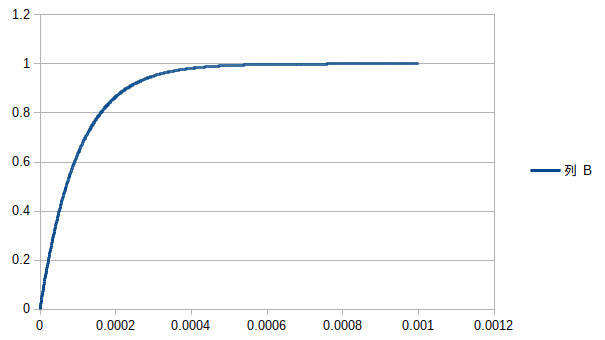
\includegraphics[width=80mm]{graph.png}
\caption{グラフの例}\label{graph}
\end{figure}


%\begin{quote}

%\begin{verbatim}



%\end{verbatim}

%\end{quote}



%%%%%%%%%%%%%%%%%%%%%%%%%%%%%%%%%%%%%%%%%%%%%%%%%%%%%%%%%

\newpage

\section*{課題1-3(応用)}

\myheader



\subsection*{説明}



ここに、課題(基礎)のソースコード、実行の様子の説明を記載。



\subsection*{考察}



ここに、課題(基礎)のソースコードのプログラミング手法や

コンピュータの動作などについて理解したこと、疑問に思ったこと、

残された課題と改善策などを記載。



\subsection*{ソースコード}



%\subsubsection*{helloworld.c}

%\lstinputlisting[basicstyle=\ttfamily\footnotesize, %frame=single]{helloworld.c}



\subsection*{実行結果}



%\begin{quote}

%\begin{verbatim}

%

%\end{verbatim}

%\end{quote}

% 参考文献挿入参考サイト
% https://www.overleaf.com/learn/latex/Bibliography_management_in_LaTeX

\end{document}